\chapter{Correlative microscopy}


\section{Combination of \acs*{SEM} - \acs*{BSE} + \acs*{EDX}}

{\color{red} relevance? usually \ac{SEM} / \ac{BSE} + \ac{EDX} do already align - Measurements with ageing specimens/ retransferred specimens}

\begin{enumerate}
  \item realignement using fiducials
  \item combination of \ac{SEM} - \ac{BSE} + \ac{EDX} + \ac{LAICPMS}
  \item combination of \ac{SEM} - \ac{BSE} + µXRF
\end{enumerate}

\section{Combination of \acs*{SEM} - \acs*{BSE} + \acs*{EDX} + µXRF + nanoindentation}

{\color{red}
TODO: Erstmal nur eine Idee - hier fehlt mir noch ein wenig der Mehrwert/Plan - Zoom in?}


nanoindentation: \cite{li.2025a,li.2025}



\section{Combination of \acs*{SEM} - \acs*{BSE} + \acs*{EDX} + \acs*{LAICPMS} }
\label{sec:corr_laicpms}

\textit{The results of this section are mostly published in \textcite{kleiner.2022b}.}

The measurements were done on an embedded and polished clinker grain.
The areas are marked in Figure~\ref{fig:LAICPMS-specimen}.
They are visible as tiny dark spots already indicating the damage induced by the laser ablation.
In total, there were three mapping areas and one spot analysis area.

\subsection{Example area 1}

The evaluation is described using one mapping position as an example.
Figure~\ref{fig:LAICPMS-positon2} shows the area of the \ac{EDX} mapping and the following \ac{LAICPMS} area on top of a \ac{BSE}-image.

\begin{figure}[htb!]
  \centering

  \ifdefined\PRINTABLE
    \includegraphics[width=.9\linewidth]{la-icp-ms/position2.pdf}
  \else
    \animategraphics[loop,autoplay,width=.9\linewidth]{.5}{figures/la-icp-ms/position2-anim/Animation}{0}{4}
  \fi
  \caption{Mapping area 2. Position of the Si-\ac{EDX}- (red) and Ba-\ac{LAICPMS}-mapping (yellow). \cite{kleiner.2021d}}
  \label{fig:LAICPMS-positon2}
\end{figure}

The areas measured contain all relevant phases, as alite, belite, \ac{C3A}, \ac{C4AF}, \ce{MgO}, \ce{CaO} and alkali sulphates.
Alite and belite are easily identifiable in the \ac{BSE} image (belite appears a little darker than alite), but also in the \ac{EDX} mappings.
The \ce{Ca}, \ce{Si}, \ce{Al} and \ce{Fe} \ac{EDX} element distribution maps marked in Figure~\ref{fig:LAICPMS-EDX}.

\begin{figure}[H]
  \centering

  \begin{subfigure}[t]{0.32\textwidth}
    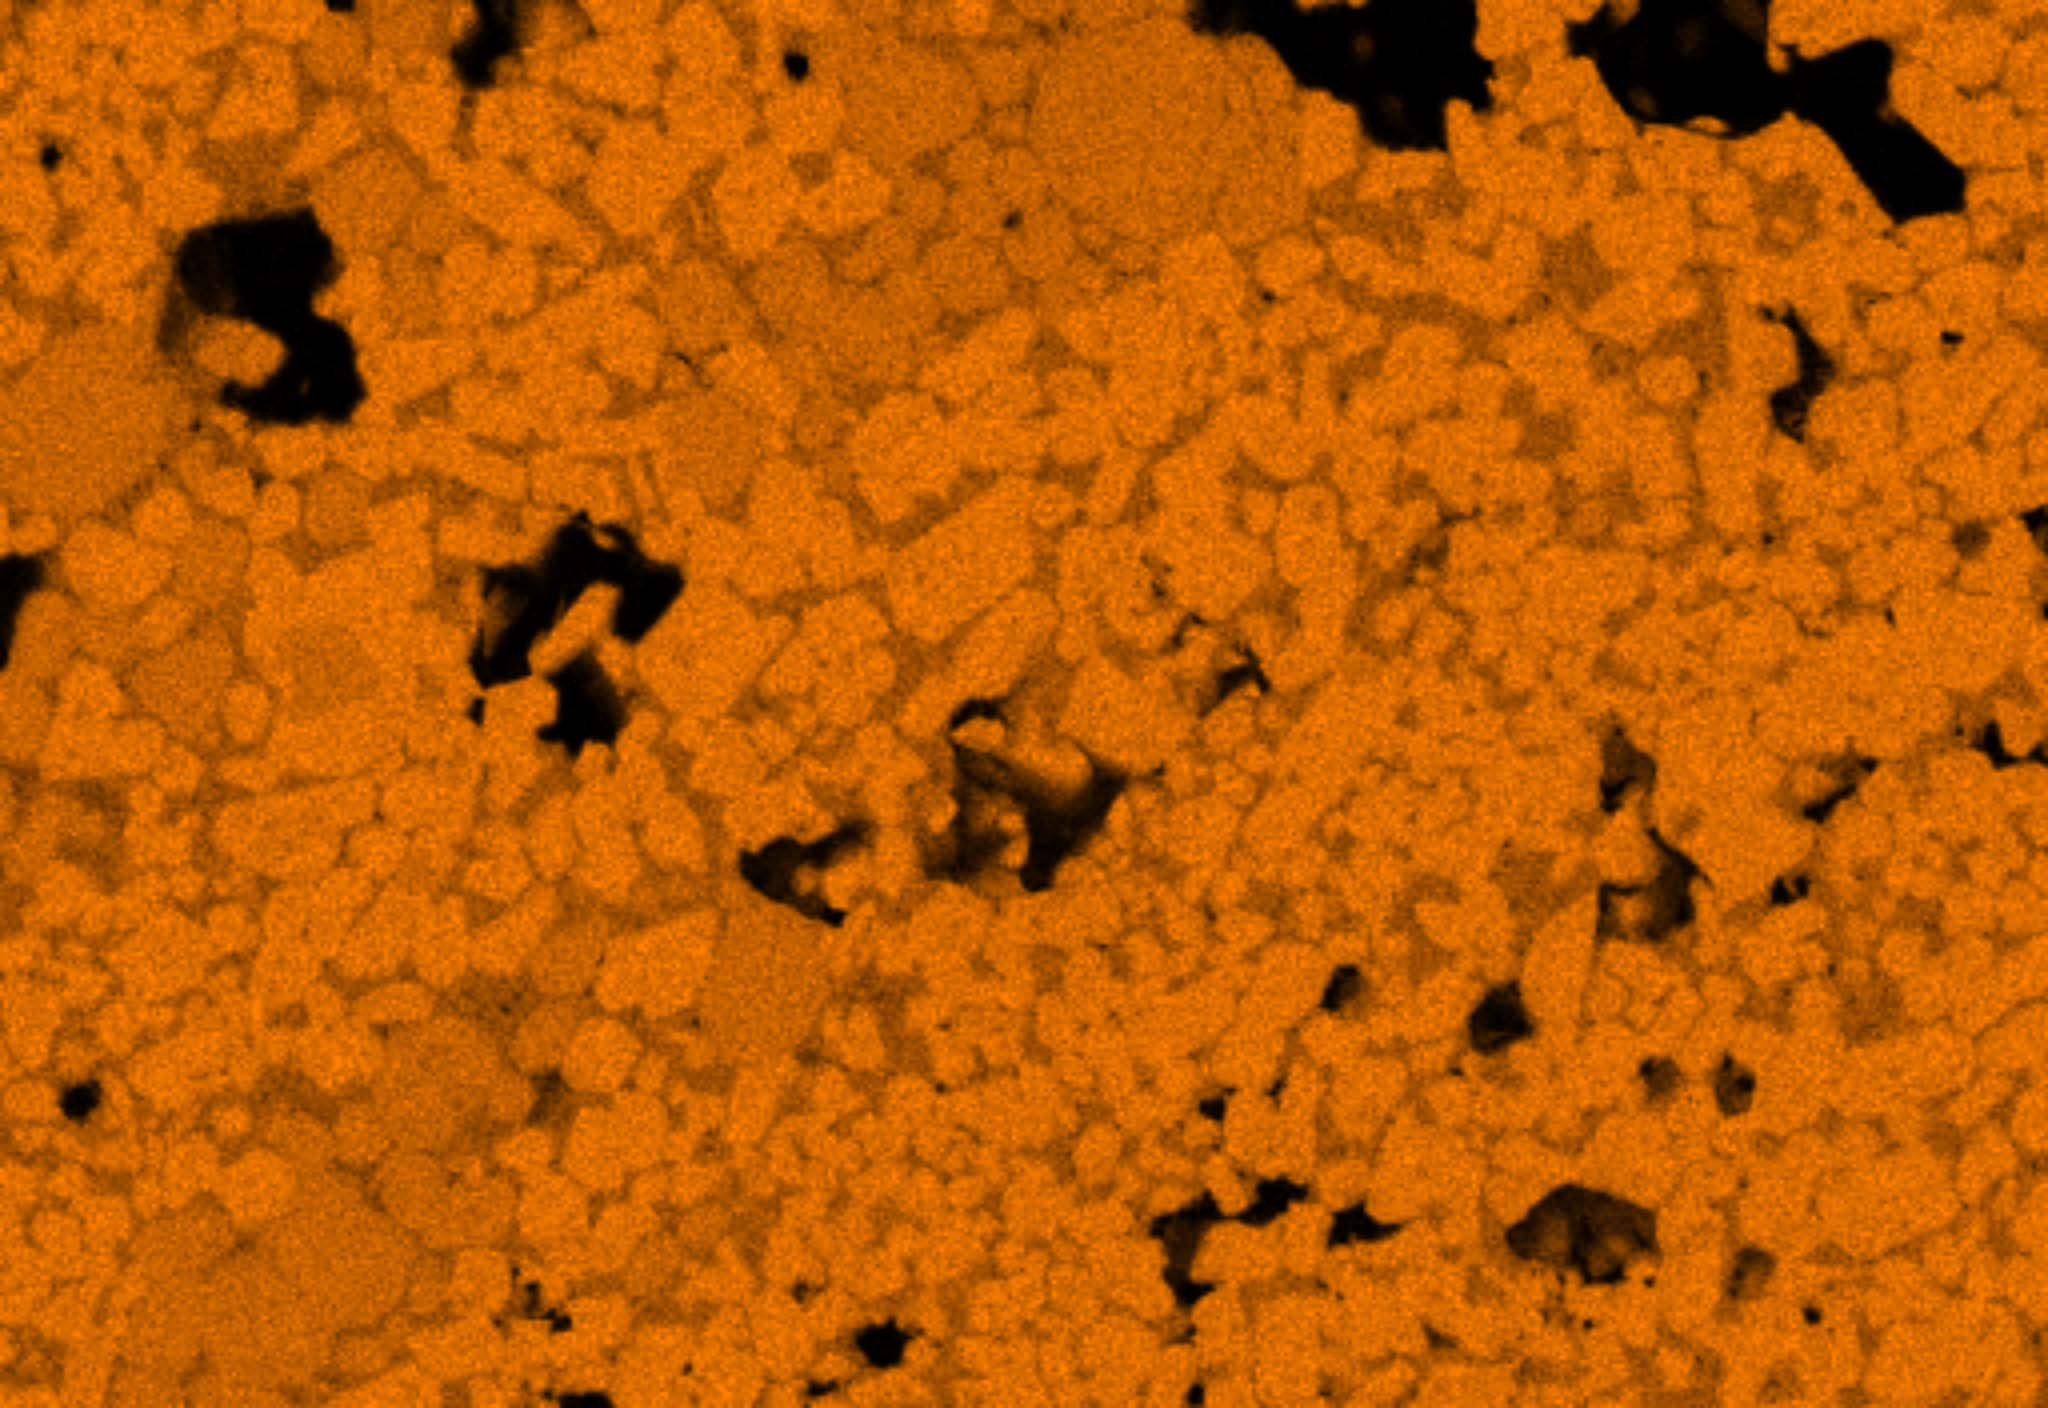
\includegraphics[width=\textwidth]{figures/la-icp-ms/edx/Ca.jpg}
    \caption{Ca mapping}
    \label{fig:LAICPMS-EDX-Ca}
  \end{subfigure}
  \hfill
  \begin{subfigure}[t]{0.32\textwidth}
    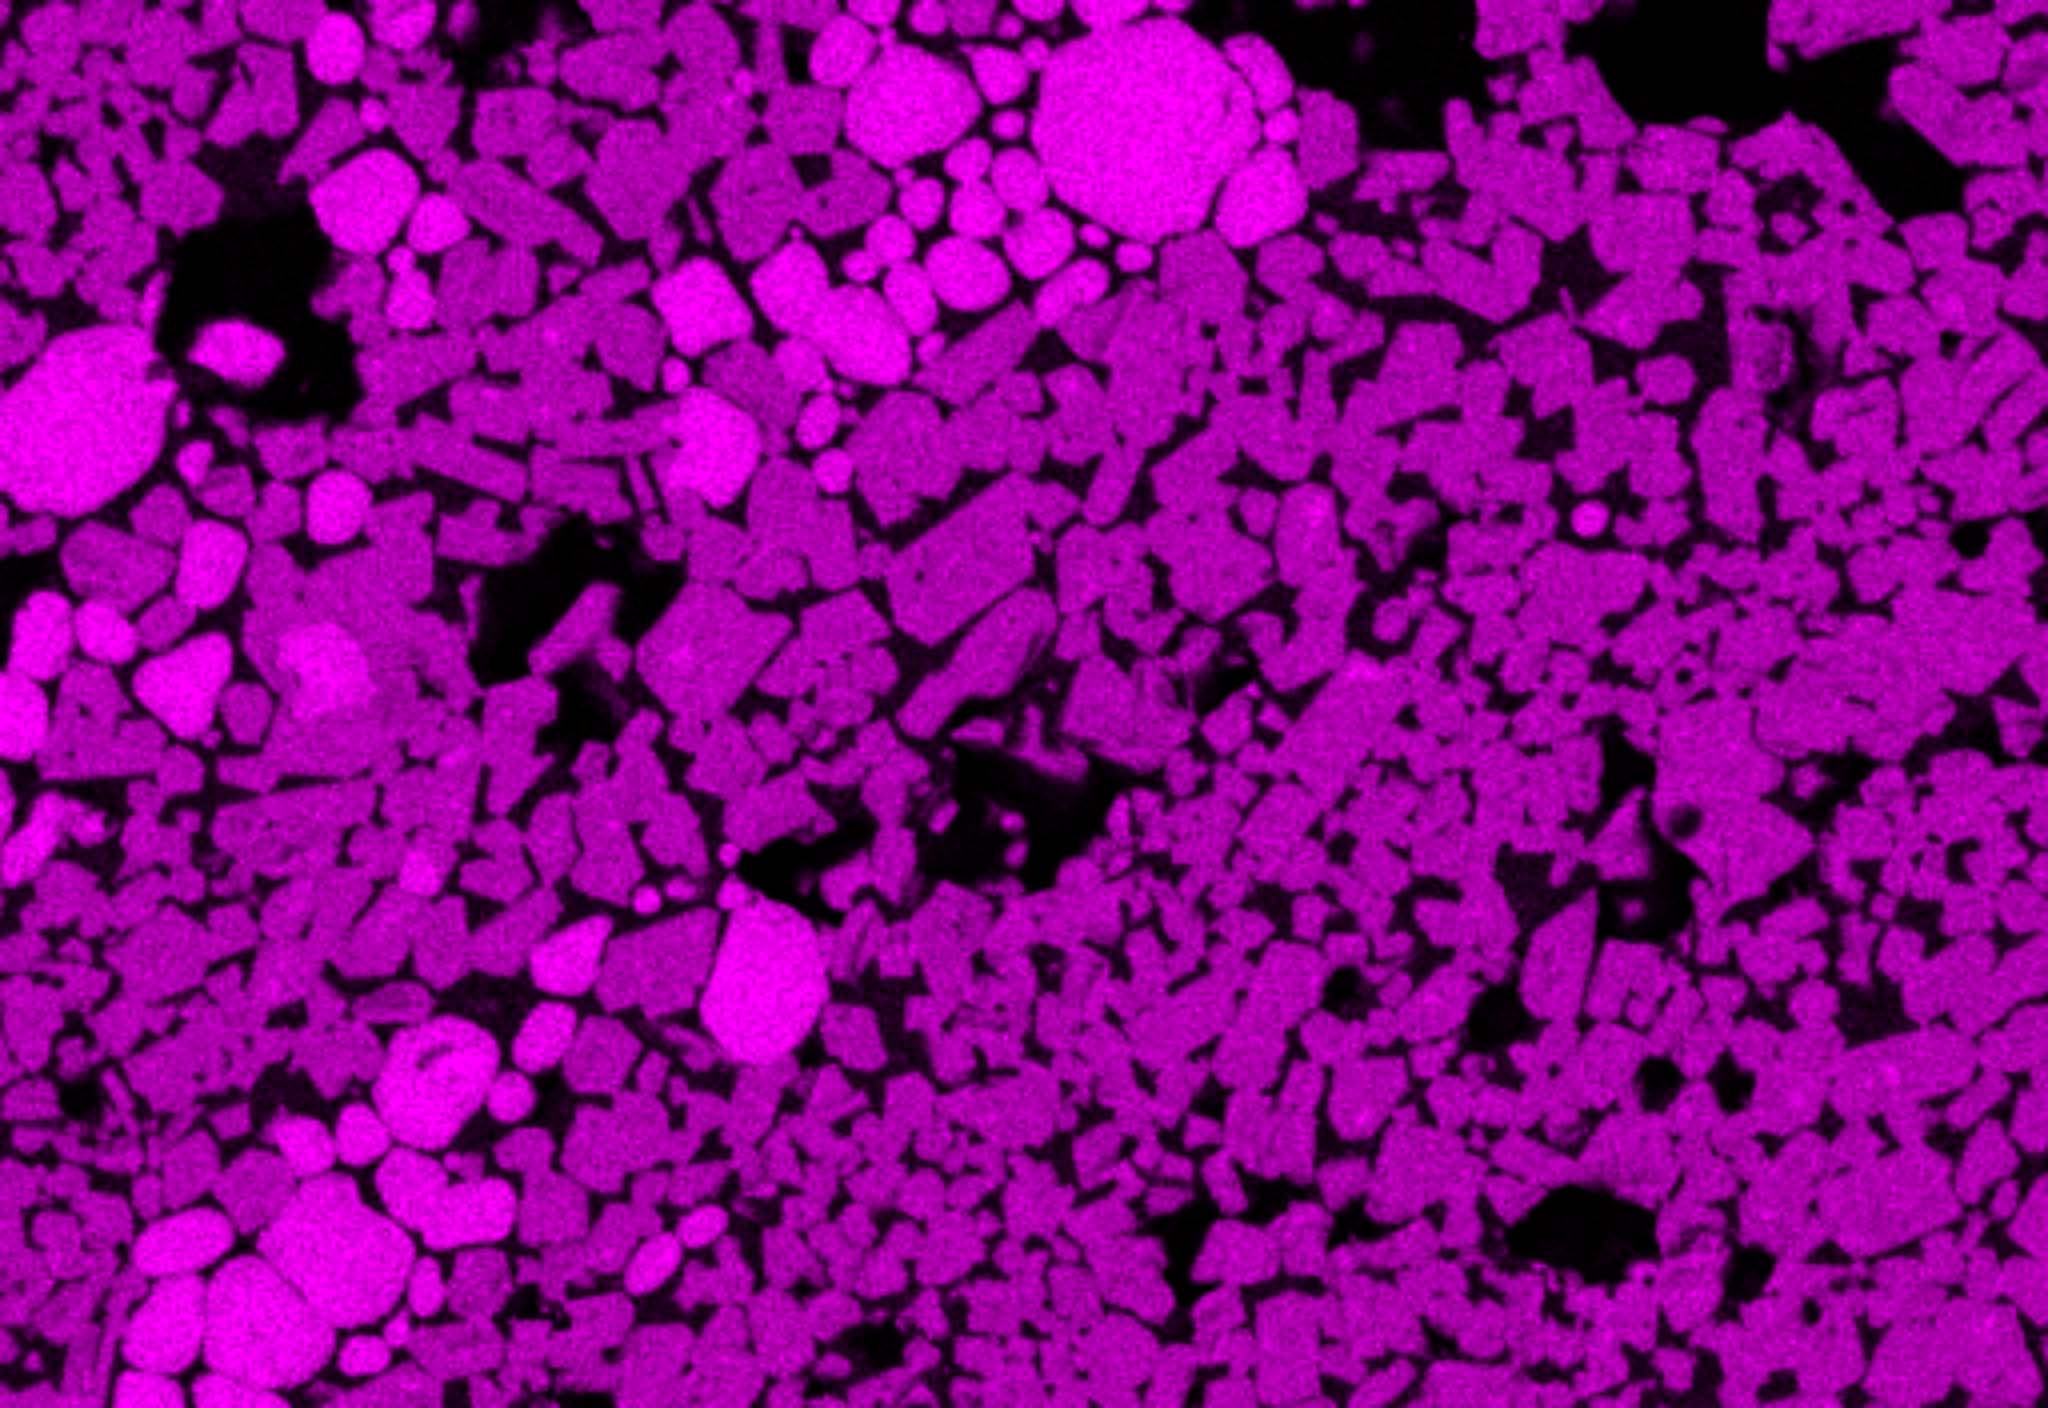
\includegraphics[width=\textwidth]{figures/la-icp-ms/edx/Si.jpg}
    \caption{Si mapping}
    \label{fig:LAICPMS-EDX-Si}
  \end{subfigure}
  \hfill
  \begin{subfigure}[t]{0.32\textwidth}
    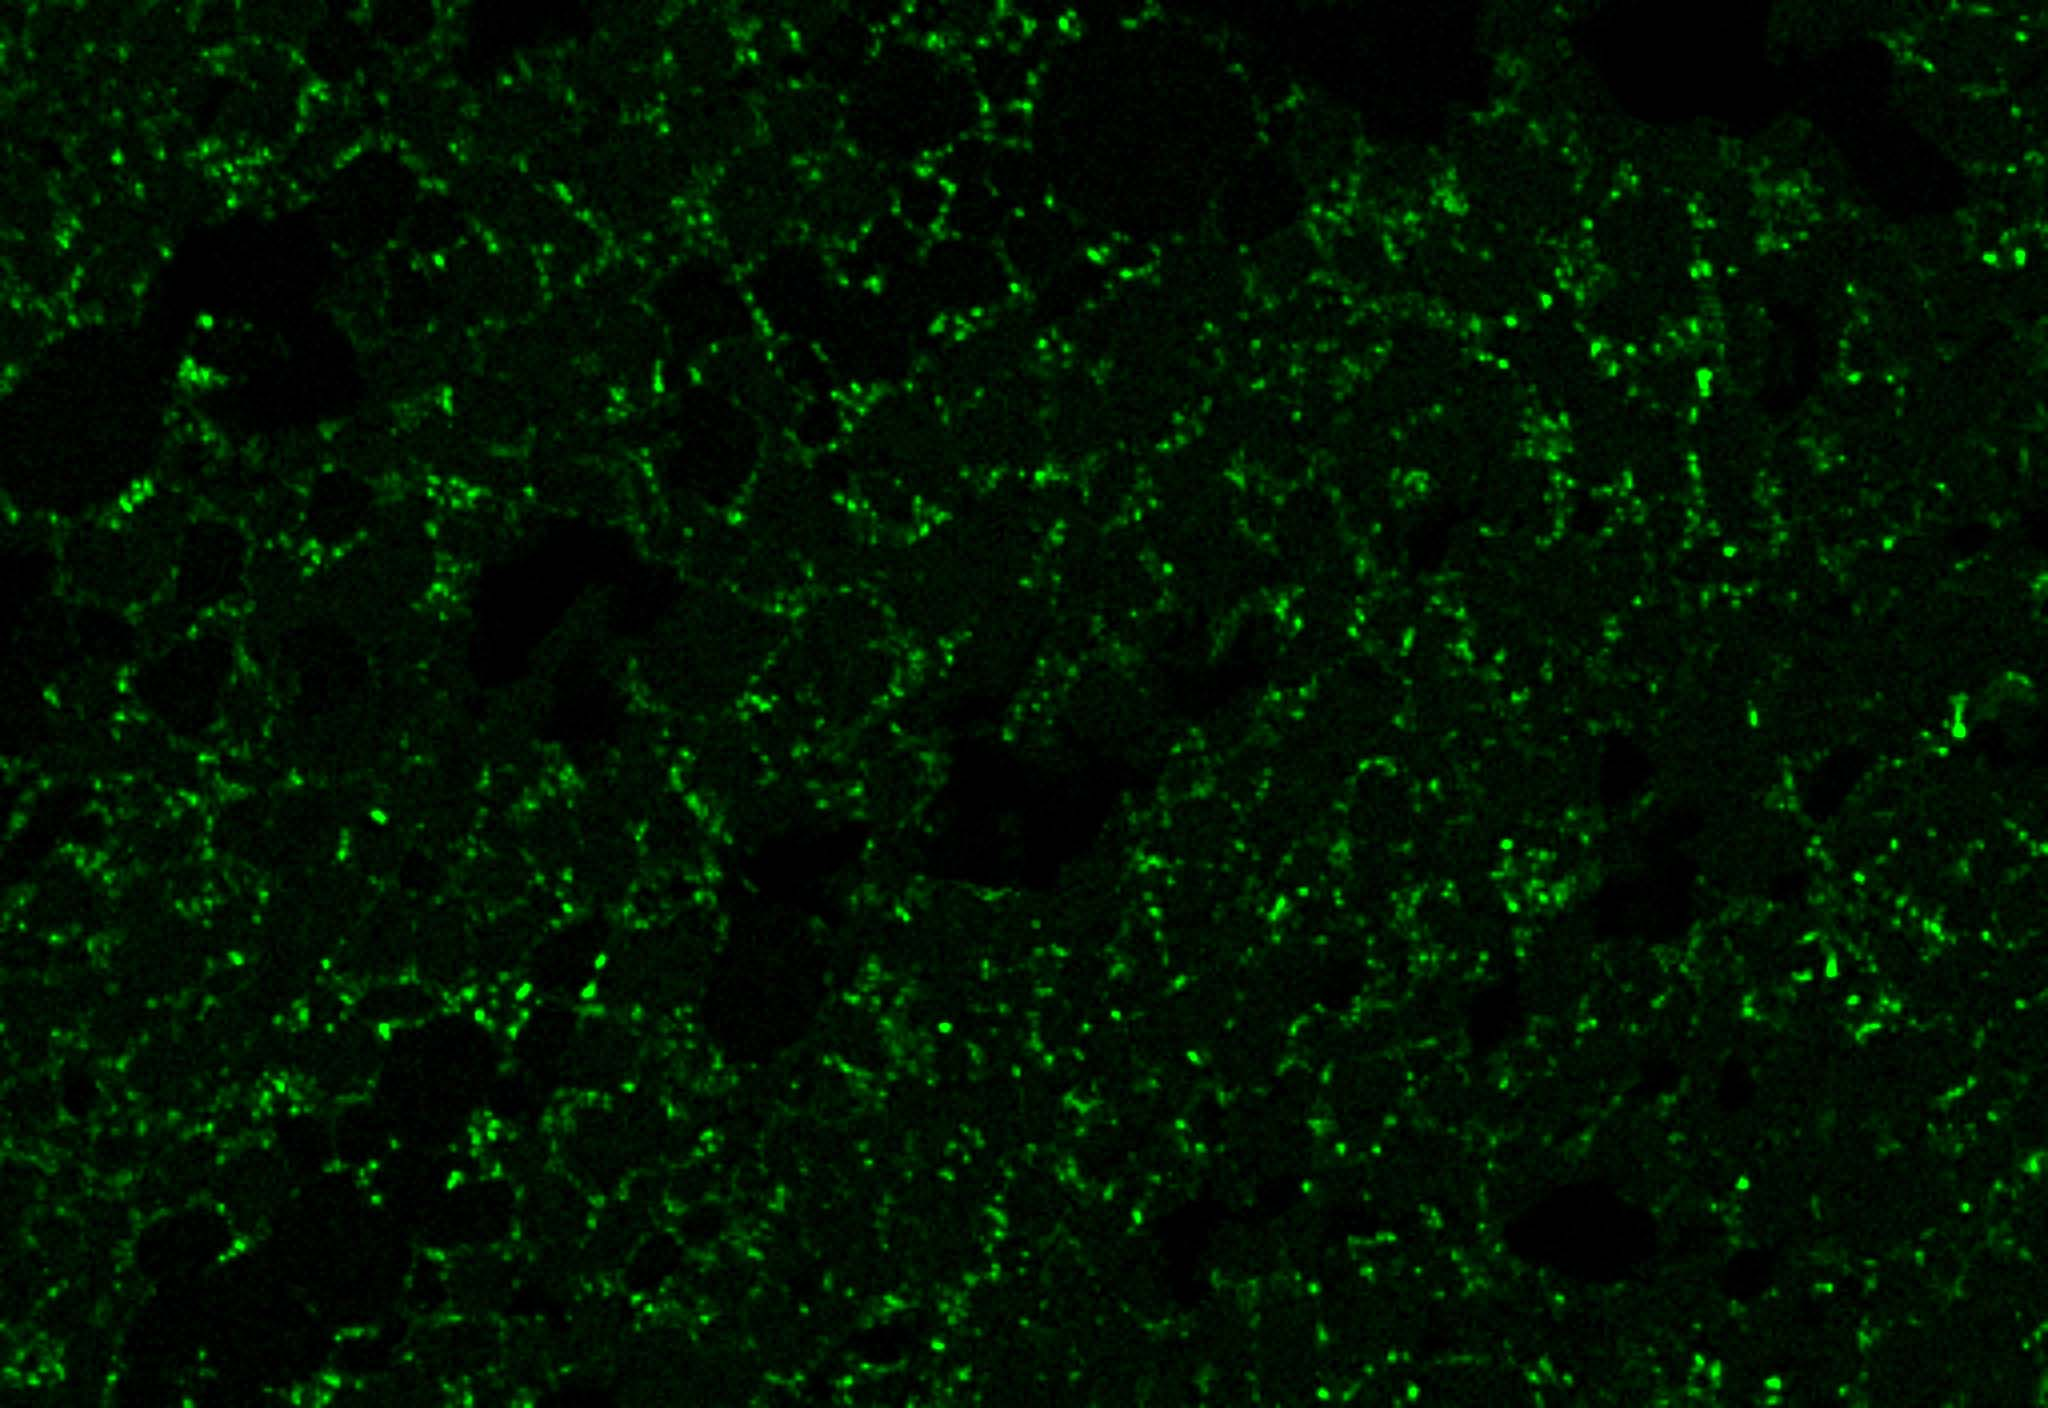
\includegraphics[width=\textwidth]{figures/la-icp-ms/edx/Mg.jpg}
    \caption{Mg mapping}
    \label{fig:LAICPMS-EDX-Mg}
  \end{subfigure}

  \begin{subfigure}[t]{0.32\textwidth}
    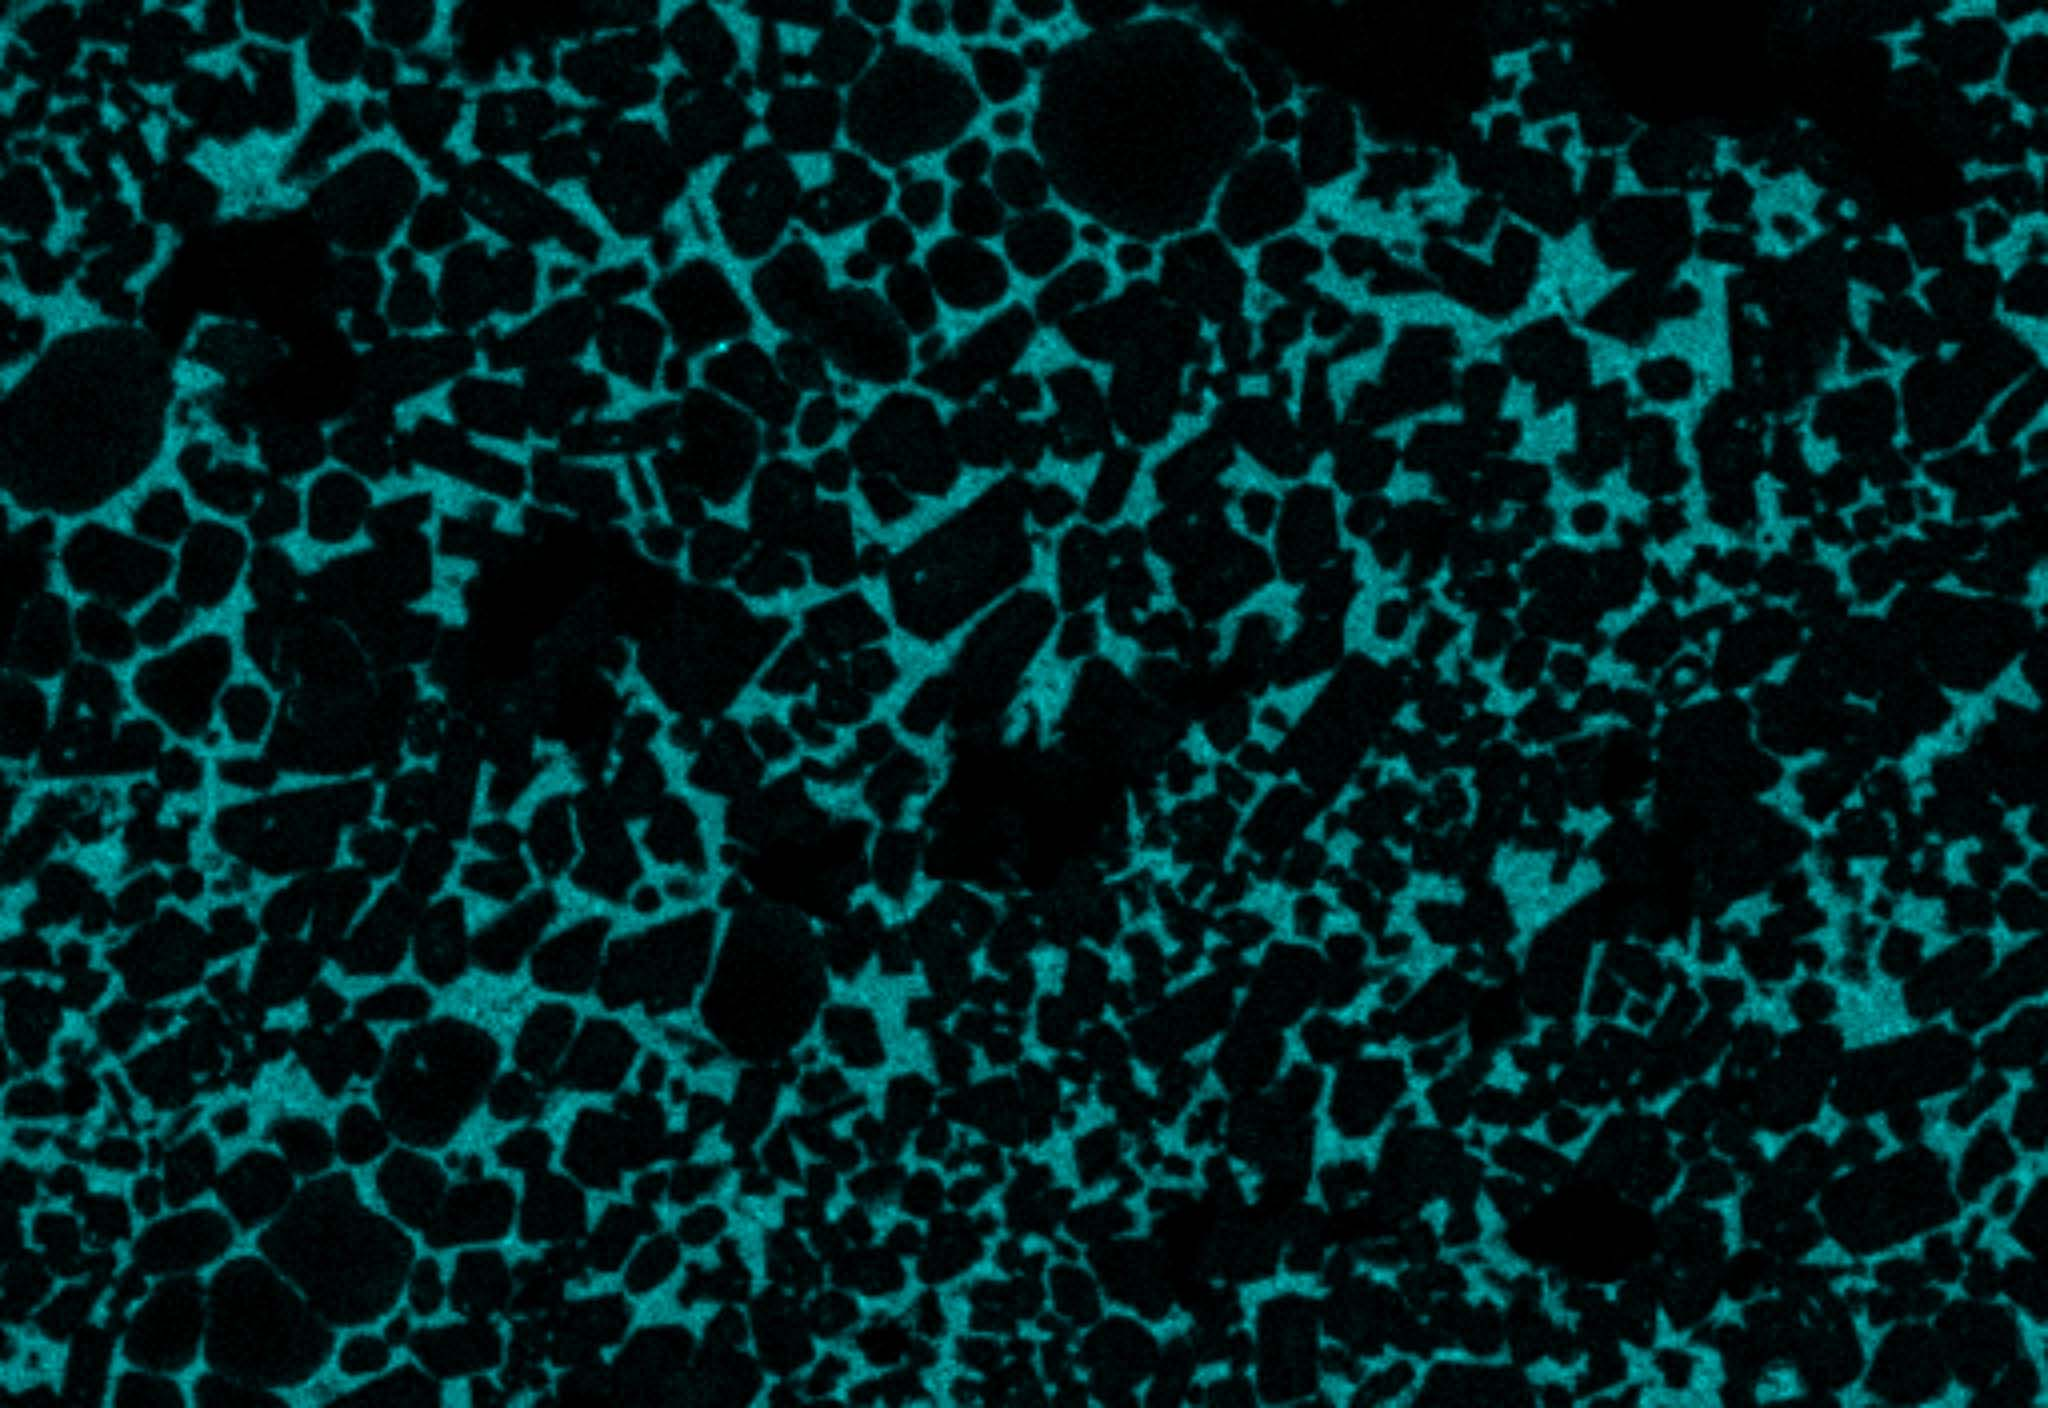
\includegraphics[width=\textwidth]{figures/la-icp-ms/edx/Al.jpg}
    \caption{Al mapping}
    \label{fig:LAICPMS-EDX-Al}
  \end{subfigure}
  \hfill
  \begin{subfigure}[t]{0.32\textwidth}
    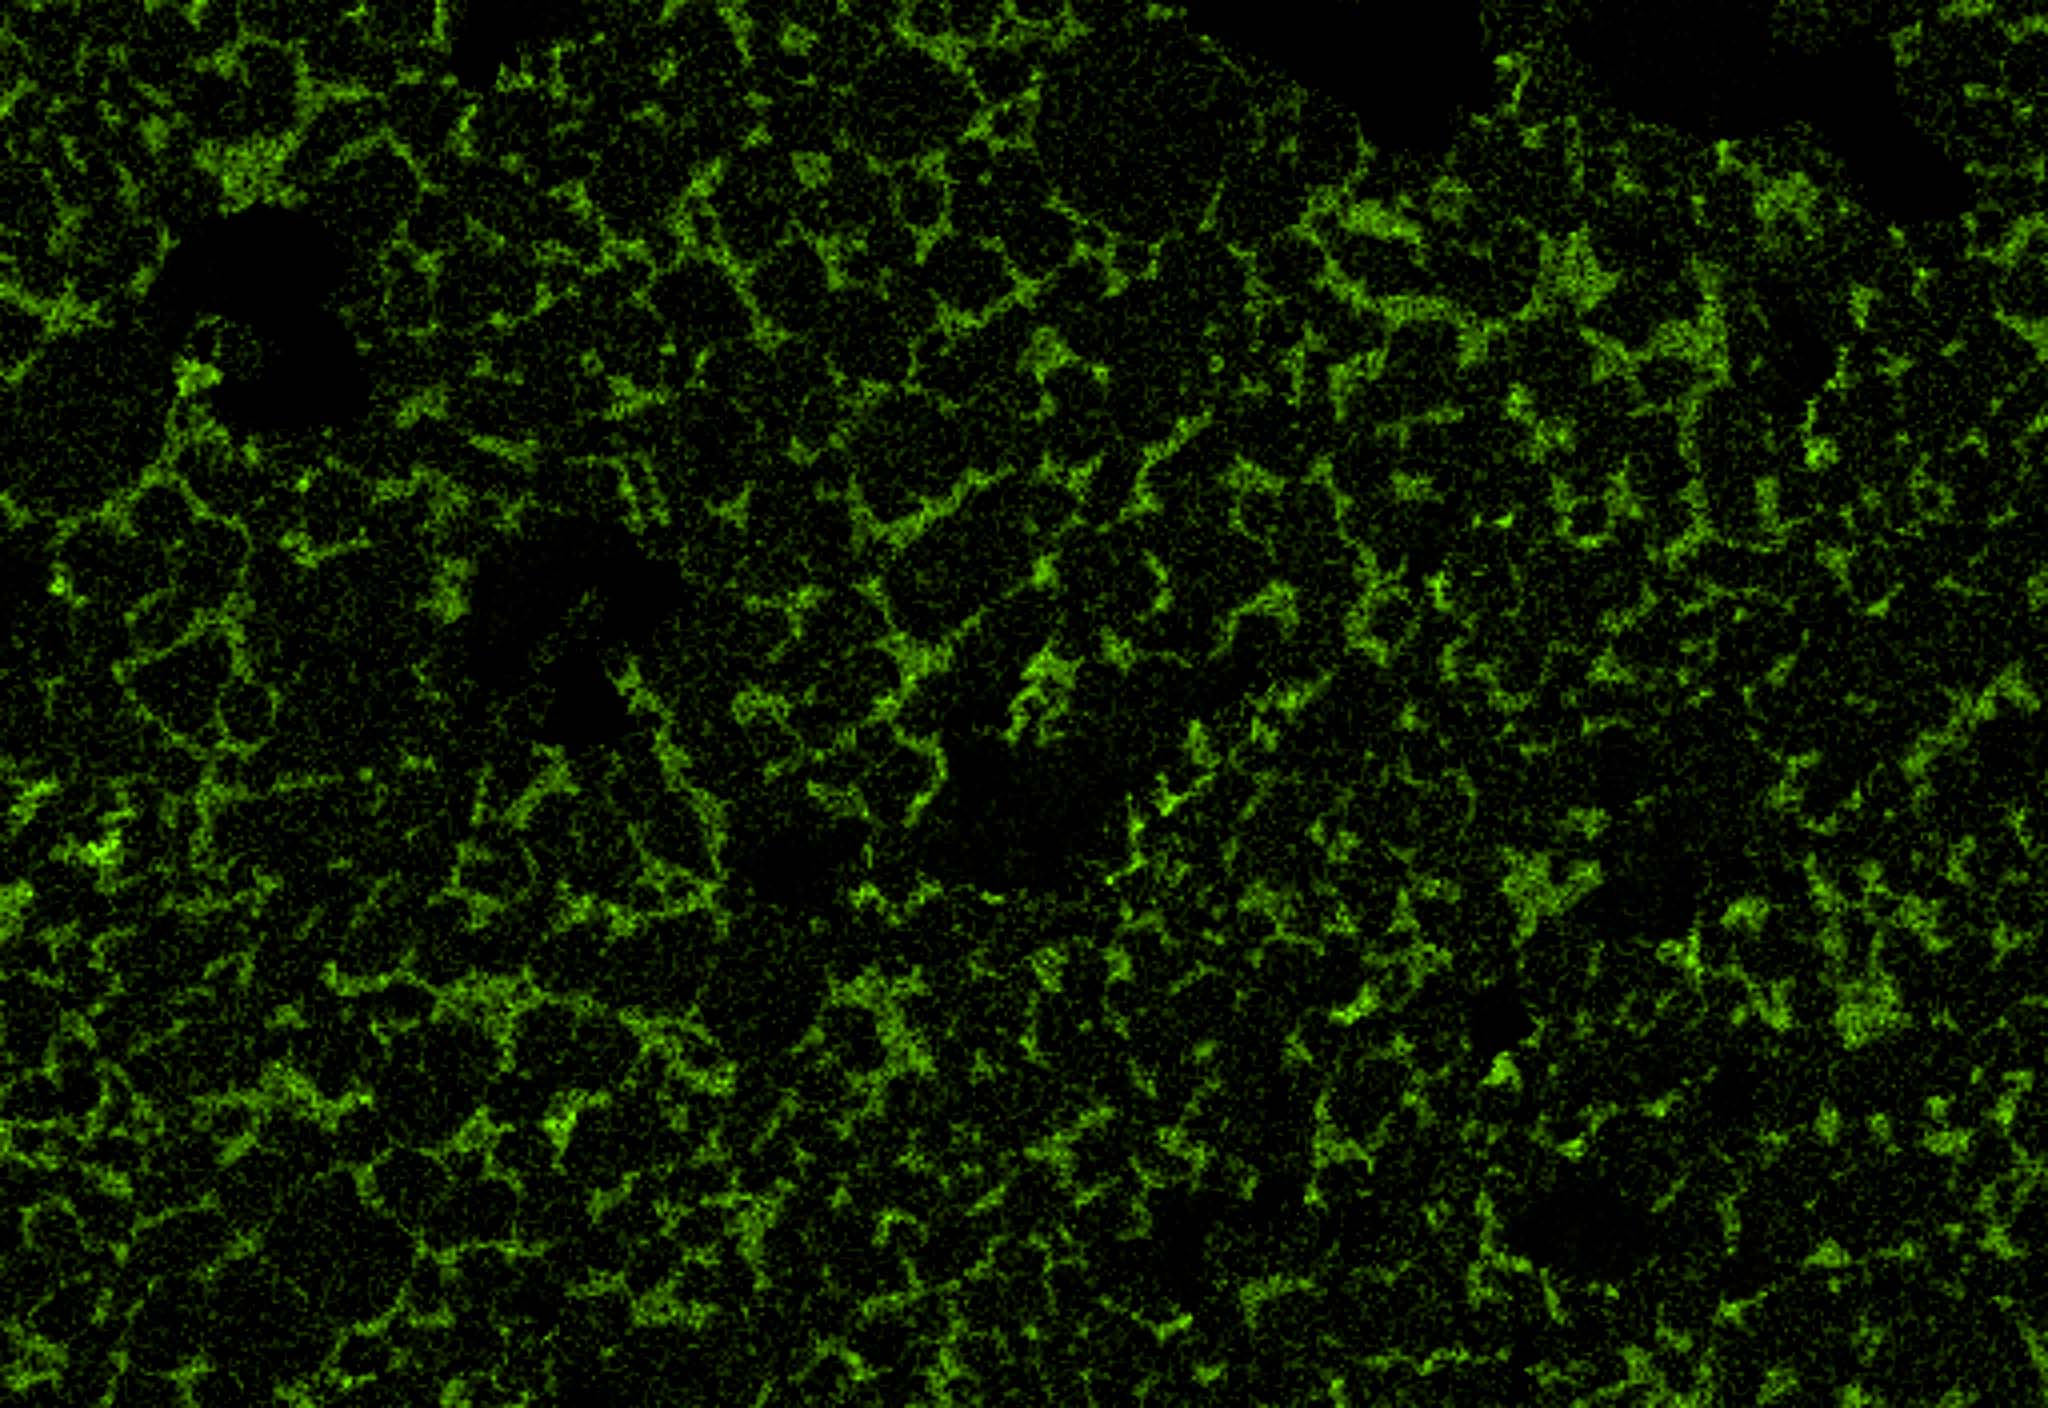
\includegraphics[width=\textwidth]{figures/la-icp-ms/edx/Fe.jpg}
    \caption{Fe mapping}
    \label{fig:LAICPMS-EDX-Fe}
  \end{subfigure}
  \hfill
  \begin{subfigure}[t]{0.32\textwidth}
    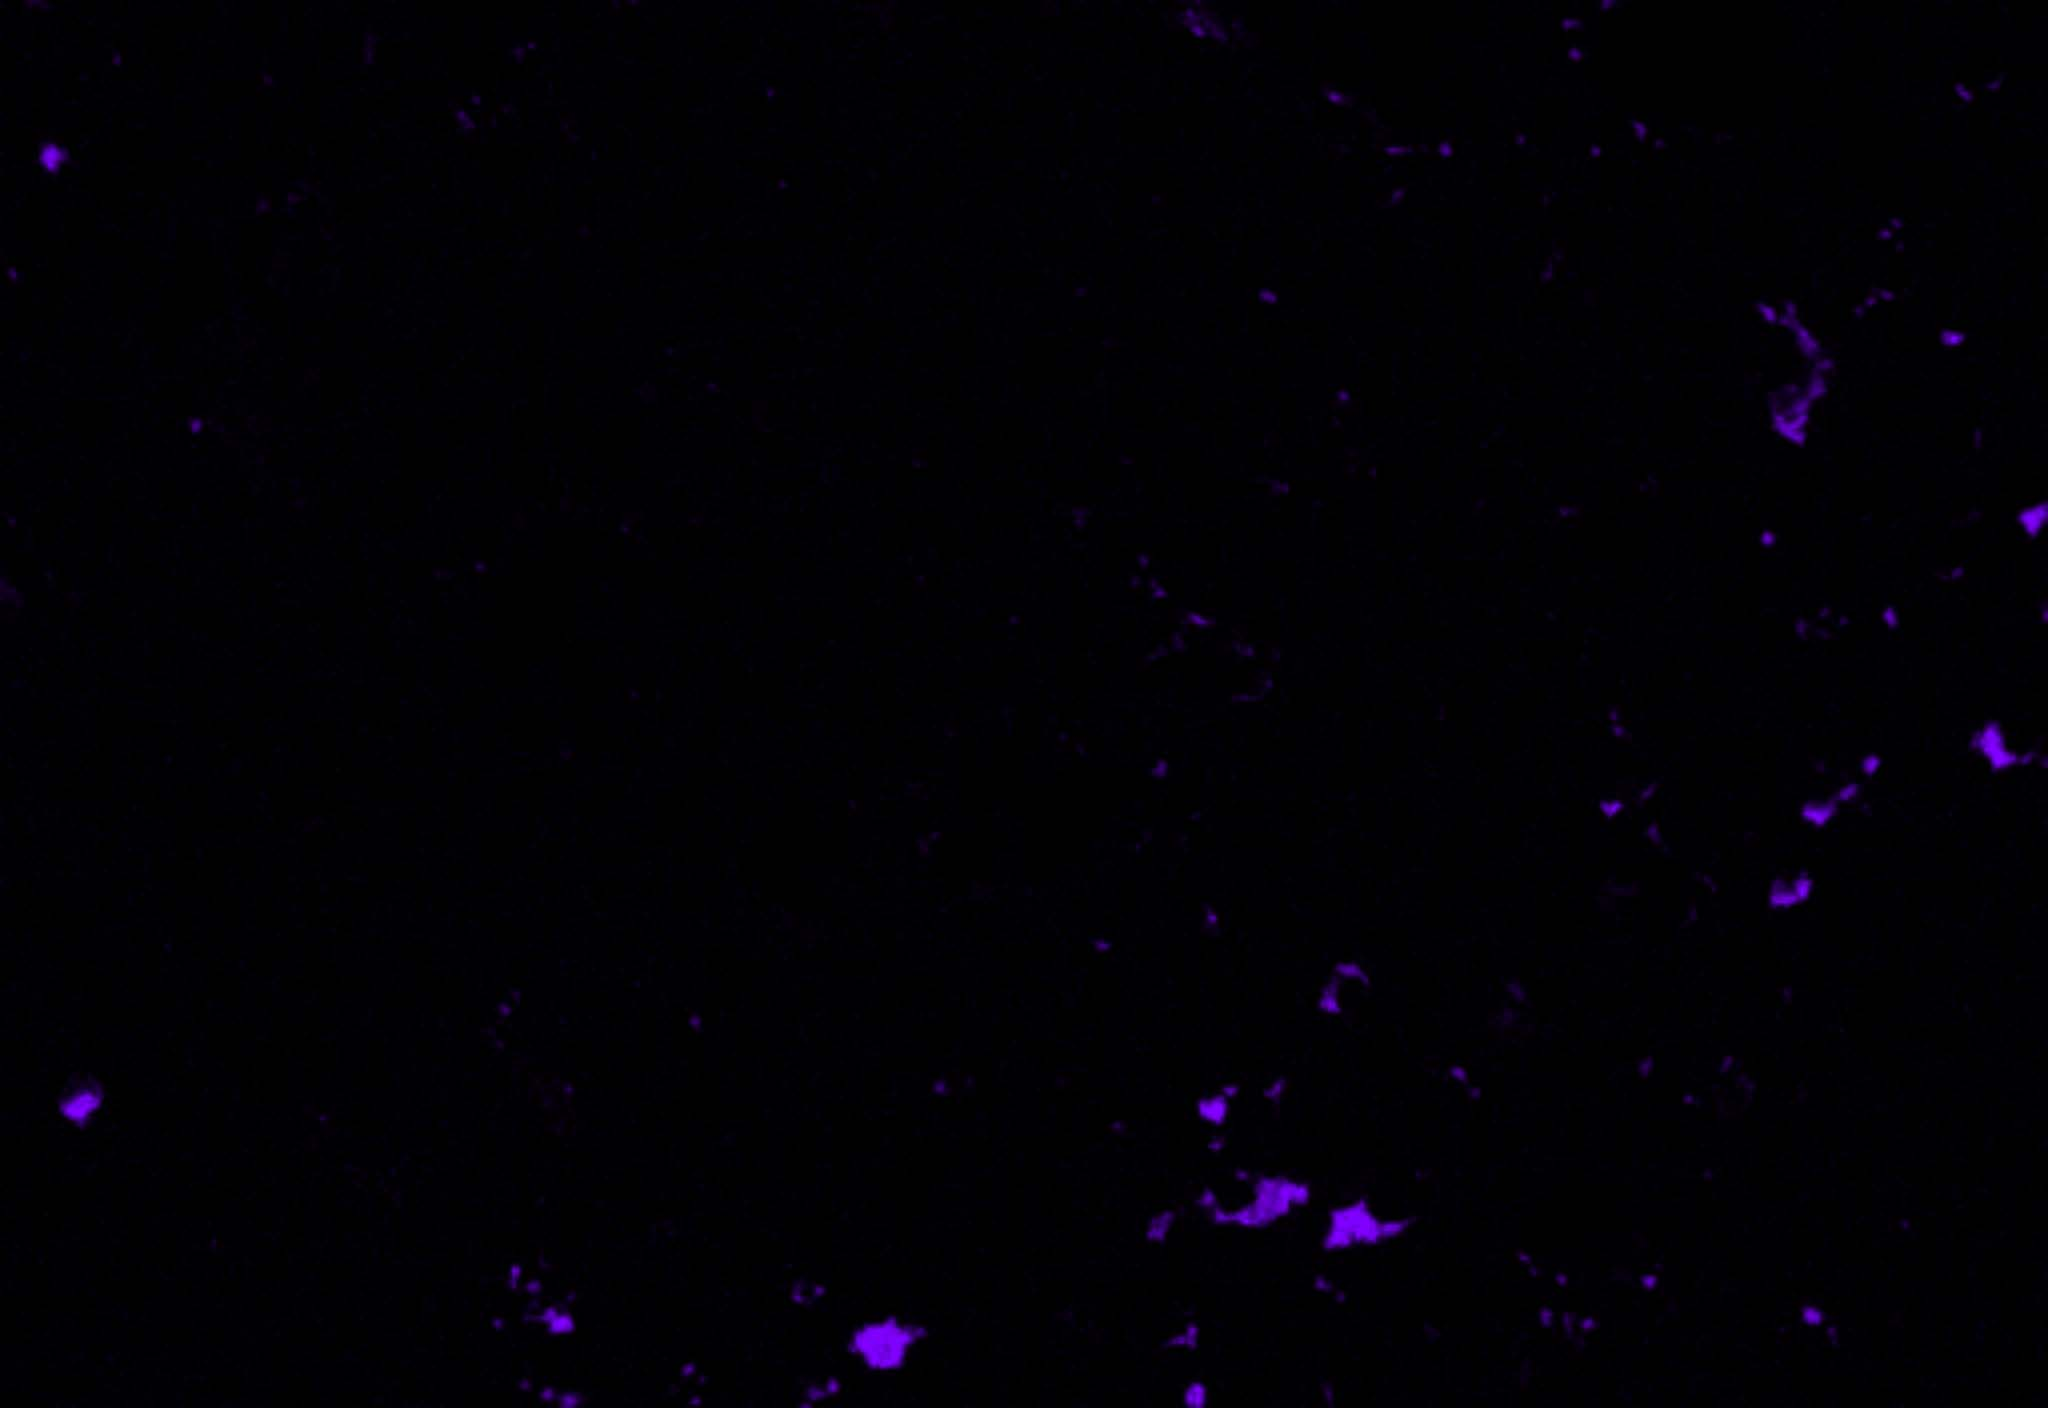
\includegraphics[width=\textwidth]{figures/la-icp-ms/edx/S.jpg}
    \caption{S mapping}
    \label{fig:LAICPMS-EDX-S}
  \end{subfigure}

  \caption{
    Element distribution maps of \ce{Ca}, \ce{Si}, \ce{Al}, \ce{Fe}, \ce{Mg} and \ce{S} of position 2, as shown in Figure~\ref{fig:LAICPMS-phasemap}.
    The images have a dimension of 260 x 179 μm.
    %Additional element distribution maps can be found in Figure S-2.
  }
  \label{fig:LAICPMS-EDX}
\end{figure}

A full phase map was calculated using the software Aztec 5.0 and the result is shown in Figure~\ref{fig:LAICPMS-phasemap}.
Comparison with the \ce{Si} element distribution map in Figure~4 reveals, that the phase map distinguished alite, belite, \ce{MgO} and alkali sulphates quite well.
\ac{C3A} and \ac{C4AF} are difficult to differentiate within the \ac{LAICPMS} dataset and are therefore combined and called `interstitial phase' from heron (marked red in Figure~\ref{fig:LAICPMS-phasemap}).

\begin{figure}[htb!]
  \centering

  \includegraphics[height=0.32\textheight]{la-icp-ms/EDX-phase-map.pdf}

  \caption{Phase map based on the \ac{EDX}-dataset (see Figure~\ref{fig:LAICPMS-EDX}). \cite{kleiner.2022b}, \ac{SI}}
  \label{fig:LAICPMS-phasemap}
\end{figure}

The belite (yellow) can be seen mainly on the left half of the image in three clusters containing less \ce{Ca} and more \ce{Si} as the alite (green).
The alumina rich interstitial phases can best be seen in the \ac{EDX}-mappings, while they usually appear as light (\ac{C4AF}) to medium grey (\ac{C3A}) in the \ac{BSE} image between the alite crystals.

The positions of the phases \ce{K2SO4} and \ce{MgO} is indicated in the \ac{EDX} mapping of \ce{Mg} and \ce{S} (Figure~\ref{fig:LAICPMS-EDX-Mg} and \ref{fig:LAICPMS-EDX-S}).
However, the \ce{MgO} phase positions are not visible in the phase map, due to their small size.
Elements like \ce{C} and \ce{Cl} can not be considered for further analysis, since they are contained in the epoxy resin.
%In contrast, the maps of \ce{Na} and \ce{Ti} are very noisy and difficult to interpret.
%These mappings can be found in Figure~S-2.

%At least for unhydrated clinker, the individual phases seemed to be damaged in a similar fashion, while the epoxy resin was ablated a lot deeper.

The elemental maps of other elements like \ce{Na}, \ce{Ti}, \ce{Cr}, \ce{Cu}, \ce{Mn} and \ce{P} are very noisy and therefore are not shown here.
Generally, elemental maps can be obtained in good quality, if the X-ray count number of the respective mappings are increased by increasing the measurement time.
However, the \ac{EDX} quality was not the major focus of this study.

\begin{figure}[!htb]
  \centering
  \begin{tikzpicture}
    \begin{semilogyaxis}[
        xtick = data,
        symbolic x coords={Ca,Si,Al,Fe,Mg,K,S,Na,Ti,P,Mn,Cr},
        table/col sep=comma,
        log origin=infty,
        width=\textwidth,
        height=8cm,
        ybar,
        bar width=10pt,
        enlarge x limits=0.07,
        ylabel={concentration in \si{\wtpercent}},
        xlabel={element},
        ytick={0.01,0.1,1,10,100},
        yticklabels={0.01,0.1,1,10,100},
        ymin=0.001, ymax=100,
        legend cell align=left,
        legend style={
            at={(0.98,0.97)},
            anchor=north east,
            column sep=1ex
        },
        legend columns=-1,
        error bars/y dir=both,
        error bars/y explicit,
        scaled y ticks = false,
        error bars/y dir=both,
        error bars/y explicit,
    ]

      \addplot[
        orange,fill=orange,
      ] table [
        x=element,
        y=c_analy_alt,
        col sep=comma
      ] {figures/la-icp-ms/chemical-edx.csv};
      \addlegendentry{\acs*{ICP}-\acs*{OES} analysis};

      \addplot[
        blue, fill=blue,
        error bars/.cd,
        error bar style={black},
      ] table [
        x=element,
        y=EDX_mean_area,
        y error=stabw_edx_area,
        col sep=comma
      ] {figures/la-icp-ms/chemical-edx.csv};
      \addlegendentry{\ac*{EDX} analysis};

      \draw [red, thick, dashed] (axis cs:Ca, 0.1) node [below, anchor=north west, align=left, text=black, fill=white, fill opacity=0.5, text opacity=1] {lower \ac{EDX} detection limit} -- (axis cs:Cr, 0.1) ;
      %\draw [red, thick, dashed] (rel axis cs:0,0.1) node [below, anchor=north west, align=left, text=black, fill=white, fill opacity=0.5, text opacity=1] {lower \ac{EDX} detection limit} -- (rel axis cs:1,0.1) ;

    \end{semilogyaxis}
  \end{tikzpicture}

  \caption{
    Comparison of the results (oxide concentrations) from the chemical analysis (\ac{ICP}-\ac{OES}; see Table~\ref{tab:laicpms-clinker}) and the \ac{EDX} analysis obtained from the sum spectra of the three mappings.
    \cite{kleiner.2022b}
  }
  \label{fig:LAICPMS-EDX-chemical}
\end{figure}

To validate the \ac{EDX} results, they were compared to the \ac{ICP}-\ac{OES} measurement (see Table~\ref{tab:laicpms-clinker}).
For this purpose, the \ac{EDX} results were averaged over the three mappings and the results were plotted in Figure~\ref{fig:LAICPMS-EDX-chemical}.
However, the \ac{ICP}-\ac{OES} results are mostly within the range of the \ac{EDX} standard deviations.
The oxide concentrations show obvious differences.
This indicates that the area analysed using \ac{EDX} is too small to be representative to obtain a chemical composition close to the \ac{ICP}-\ac{OES} results.
Concentrations below \SI{0.1}{\wtpercent} oxide are outside of the \ac{EDX} detection limit - this concerns the elements \ce{Na}, \ce{P}, \ce{Mn} and \ce{Cr}. 

\begin{figure}[htb!]
  \centering

  \ifdefined\PRINTABLE
    \includegraphics[width=.9\textwidth]{la-icp-ms/la-icp-ms-mapping/result0.pdf}
  \else
    \animategraphics[loop,autoplay,width=.9\textwidth]{1}{la-icp-ms/la-icp-ms-mapping/result}{0}{2}
  \fi

  \caption{
    Element distribution maps generated by \ac{LAICPMS}.
    The images cover an area of \num{483.8} $\times$ \SI{343.4}{\micro\meter\squared} using \num{80} $\times$ \num{603} measurements.
    The outlines for alite (black) and belite (white) were derived from the \ac{EDX}-phase map shown in Figure~\ref{fig:LAICPMS-phasemap}. \cite{kleiner.2022b}, \ac{SI}
  }
  \label{fig:LAICPMS-la-maps}
\end{figure}

Results in Figure~\ref{fig:LAICPMS-la-maps} show the element distribution maps obtained by \ac{LAICPMS}.
Some elements show regions of very high concentrations, which are called hotspots in this article.

Compared to the \ac{EDX} element distribution maps shown in Figure~\ref{fig:LAICPMS-EDX}, the \ac{LAICPMS} maps possess a lower spatial resolution.
When the \ce{Al} element distribution maps obtained by both methods are compared (Figures~\ref{fig:LAICPMS-EDX} and \ref{fig:LAICPMS-la-maps}), it is revealed that \ac{LAICPMS} is not able to sharply represent the phase boundaries between the finely grained interstitial phase (\ac{C3A} and \ac{C4AF}) phases and the silicate phases.
However, the differences in the element distribution between alite and belite are very noticeable.
I.e., the \ce{Ba}, \ce{Rb} and \ce{V} mappings show a significant concentration variation in both phases.
Nevertheless, for the interstitial phase an enrichment of selected elements is notable.
While high \ce{Al} concentrations are expected, the mappings also reveal an accumulation of \ce{Mn}, \ce{Rb} and \ce{K}.
\color{blue}
Thus, it can be assumed that both alkali metals are enriched in the same phase.
As shown by \ac{EDX} element and deduced phase maps (Figures~\ref{fig:LAICPMS-EDX}, 5 and Figure~S 2), \ce{K} is associated with \ce{S}.
Therefore, it is concluded that \ce{Rb} is incorporated in \ce{K2SO4}.
This may be due to the equivalent ionic character (+1). However, also \ce{Cr}, \ce{V}, \ce{Zn} seem to be prominent in the same hotspots, despite of their highly different atom size and oxidation number.

In contrast to \ac{EDX}, \ac{LAICPMS} has lower detection limits for most of the elements.
However, the spatial resolution is too low to exactly quantify concentrations in phases that are in the size of the laser ablation spot size, such as \ac{C3A} and \ac{C4AF}.
Nevertheless, by combining the phase segmentation, acquired using the \ac{EDX}-mapping data, with the \ac{LAICPMS} data (Figure~\ref{fig:LAICPMS-la-maps}), the main clinker phases alite and belite and interstitial phases like \ac{C4AF} and \ac{C3A} may be analysed, even though this analysis may be inaccurate due to several reasons, which are discussed in the following.
Comparison of \ac{EDX} and \ac{LAICPMS} quantification results for the interstitial phase are shown in Figure~8.
For example, the \ce{Al} content measured by \ac{EDX} and \ac{LAICPMS} -mappings at the same locations varies significantly, e.g. \ac{EDX} \SI{23.1}{\wtpercent} and \ac{LAICPMS} \SI{7.8(4.2)}{\wtpercent}.
The lower value for \ac{LAICPMS} might origin from inaccurate registration of both data sets, inaccurate calibration or most probably the phase variation due to the z-effect. Nevertheless, obtained concentrations (\ce{Al}, \ce{Mg}, \ce{Ti}, \ce{K}, \ce{Na}, \ce{Mn}, Figure~8) always have the same order of magnitude.
Therefore, it can be assumed that the registration result is reliable. For the same area the presence of the following trace elements (i.e. <\,\SI{0.1}{\wtpercent}) could be proven by \ac{LAICPMS}: \ce{Ba}, \ce{Zn}, \ce{Cr}, \ce{V}, \ce{Rb} (Figure~7 and 8).
The quantified concentrations are similar for all analysed clinker areas (see supplementary document).
For area 3 (Figure~S-22) also the Si concentration of the interstitial phase was measured by \ac{LAICPMS}.
Results show that by \ac{EDX} the Si content is lower, and the \ce{Al} content is higher than concentrations given by \ac{LAICPMS} (Figure~S-22).
This can be seen as hint that due to the larger spot size the laser ablation results are more deviated by neighbouring silicate phases than \ac{EDX} analysis.
Reversely, this results in the observed low \ce{Al} concentration (Figure~8 and Figure~S-22).
These findings proof that the laser spot size is too large to quantitatively analyse the interstitial phases. Nevertheless, enrichment of for example Mn in the interstitial phase can be proven by \ac{LAICPMS}.
Furthermore, an inaccurate image registration seems to be a minor problem, as the same trends in major, minor and trace element concentration can be found in all investigated areas (compare Tables~S-1 to S-6).

\section{\acs*{LA-ICP-MS} spot analysis}

In addition to \ac{LAICPMS} and \ac{EDX} mapping data, spot analyses have been collected on sites that were selected based on the \ac{EDX} element distribution maps.
The prerequisite for selecting sites for spot analyses was that the area should be large enough to ensure that the laser spot ablates only a single phase.
Therefore, the laser ablation spots are re-allocated on the \ac{BSE} image and the \ac{EDX} phase map (Figure~9). Obviously, the spots for belite were more successfully placed in large homogeneous areas than for alite.
The reason is the smaller size of alite crystals.

For the spot analysis, more elements could be measured as the signal to noise ratio is drastically increased when the spot size is enlarged from approximately \SI{36}{\micro\meter\squared} (square shape) to \SI{415}{\micro\meter\squared} (round shape).
Thus, \ac{Pb}, \ac{Ni}, \ac{As}, \ac{Sr}, \ac{Cu} and \ac{P} could be measured additionally in the spot analysis.
However, other trace elements like \ac{Hg} and \ac{Sb} still cannot be measured because of their extremely low concentration even if it would be possible to further enlarge the spot size to improve the detection limit.

There are rather large deviations between mapping and spot analysis for most of the elements in alite and belite (Figure~10 and 11).
Besides different calibration methods, another reason for this deviation is most likely the effect that during spot ablation more area from neighbouring phases is analysed than in mapping mode (larger spot size).
Furthermore, the \ac{LAICPMS} results are further deviated due to the $z$-effect, e.g. by material that is ablated from a certain depth.
This $z$-effect is also occurring in \ac{EDX} analysis but for the used \SI{12}{\kilo\volt} acceleration voltage the excitation volume diameter is not larger than \SIrange{1.6}{2.0}{\micro\meter}, depending on the material. Therefore, both \ac{EDX} and \ac{LAICPMS} are often affected by neighbouring phases in 3 dimensions, if the phase size is similar or smaller than the analysed sample volume.
Figure~10 and 11 show the quantitative element concentrations for alite and belite obtained from segmented mappings (given in \si{\wtpercent} oxide) and from spot analyses. The following element concentrations were determined by both methods (Al, Mg, Ti, K, Na, Mn).
The Al content in alite, as documented by results in Figure~10, as determined by \ac{SEM} -\ac{EDX} spot analysis is \SI{1.5(0.4)}{\wtpercent}, by \ac{SEM} -\ac{EDX} mapping \SI{1.5(0.0)}{\wtpercent} and by \ac{LAICPMS} mapping \SI{4.30(2.88)}{\wtpercent} respectively \ac{LAICPMS} spot analysis: \SI{2.10(0.74)}{\wtpercent}.
The deviation between \ac{EDX} and \ac{LAICPMS} seems rather large and is probably mainly caused by the effect of neighbouring phases, e.g. more Al from interstitial phase is detected by the \ac{LAICPMS} analysis.

However, the spot analysis resembles the results shown by the \ac{LAICPMS} -mappings, both results reveal the accumulation of trace elements in clinker phases.
Based on the \ac{LAICPMS} mappings it was shown that alite contains more Ba, V and Rb.
This is confirmed by spot analyses for Ba and V but not for Rb (Figure~10 and 11).
But standard deviation of Rb and most other element concentrations determined by \ac{LAICPMS} is larger for alite than for belite.
This indicates that alite concentrations are, due to smaller crystal sizes, more affected by neighbouring phases (e.g. hotspots that contain Rb in high concentration) than belite.

Barium is taken as an example to furthermore interpret the data of the mapped images and the spot analysis.
In the upper elemental distribution maps, it is clearly visible that Ba is enriched in belite (Figure 7).
Additionally, some local spots of higher concentrations can be found between the alite grains, possibly in the interstitial phases (Figure~7). The mapping data shown in Figure~10 and 11 underline the semi-quantitative observation documented in Figure~7.
For alite, the determined \ac{LAICPMS} Ba concentrations are \SI{0.0187(0.0113)}{\wtpercent} (mapping) and \SI{0.0089(0.0040)}{\wtpercent} (spot analysis).
The belite shows higher Ba concentrations, e.g. \SI{0.0351(0.0145)}{\wtpercent} (mapping) and \SI{0.0291(0.0019)}{\wtpercent} (spot analysis).
Thus, 2-times (mapping) and 3-times (spot) higher Ba concentrations are found in belite than in alite.
Ba is also detected in areas of the interstitial phase, e.g. together with high Al content (mapping, Figure~7 and 8).
For the interstitial phase (\ac{C3A} and \ac{C4AF}) the Ba concentration is between that of alite and belite (\SI{0.0234(0.0139)}{\wtpercent}).
But as seen from mapping data in Figure~7 the Ba in the interstitial phase is not as homogeneously distributed as in belite.
A more detailed analysis is necessary to reveal the incorporation of Ba in the interstitial phase.
Here it can be stated that also heterogenous distributions of trace elements in clinker phases can occur.

For major and minor phases, a comparison to \ac{SEM} -\ac{EDX} data shows the limited accuracy of \ac{LAICPMS}.
Therefore, a combination with \ac{SEM} -\ac{EDX} should be considered if major and minor elements are of interest.
In a second and third dataset, at a different area on the same polished clinker grain, the described method combination of \ac{LAICPMS} and \ac{SEM} -\ac{EDX} was repeated.
All data can be found in the supplementary document. Therein, the same results and tendencies can be found as above described.
The enrichment of elements in alite, belite and the interstitial phase (\ac{C3A} and \ac{C4AF}) measured wit \ac{LAICPMS} is visualised in Figure~12.
The results demonstrate the repeatability of the described phase segmentation method for the \ac{LAICPMS} dataset based on the \ac{SEM} -\ac{EDX} data.

Furthermore, while smaller phases could not be reliably segmented in all datasets, the enrichment of Cr and Rb in the water-soluble potassium sulphate phases is still visible in the first and the second measuring site.


\color{black}